\documentclass[12pt]{article}
\usepackage{algos-tasks}

\def\pixels{
  {2,0,0,0,0,0,0,0},
  {0,3,0,0,0,0,0,0},
  {0,3,2,1,1,0,0,0},
  {0,3,2,2,2,1,1,0},
  {0,3,2,0,0,1,0,0},
  {0,0,0,0,0,1,0,0},
  {0,0,0,0,0,1,0,0},
  {0,0,0,0,0,0,0,0}%
}

\def\pixel{
  {0,0,0,0,0,0,0,2},
  {0,0,0,3,3,3,3,0},
  {0,0,0,2,2,2,0,0},
  {0,0,0,0,2,1,0,0},
  {0,0,0,0,2,1,0,0},
  {0,1,1,1,1,0,0,0},
  {0,0,0,0,1,0,0,0},
  {0,0,0,0,0,0,0,0}%
}

\def\gridpix{
  {2,0},
  {1,3}%
}
\definecolor{pixel 0}{HTML}{3CB44B}
\definecolor{pixel 1}{HTML}{FFE119}
\definecolor{pixel 2}{HTML}{E6194B}
\definecolor{pixel 3}{HTML}{4363D8}

\usepackage{tkz-euclide}

\begin{document}
\task[regular]{Grid Rotation}

\begin{question}
In the field of computer graphics, a {\em blit} ({\em {\bfseries bl}ock {\bfseries t}ransfer}) is a low-level operation, which takes in a rectangular block of pixels from a pixel map and copies the block to some location in a different pixel map. You may assume that each blit operation takes constant-time. 

A blit can be defined by the top left and bottom right cells; that is, copy the subgrid bounded by \((x_1, y_1), (x_1+m, y_1+n)\) on one grid to the subgrid bounded by \((x_2, y_2), (x_2+m, y_2+n)\) on a second grid. This copies the first subgrid into the second subgrid componentwise, maintaining the relative positions of the cells; overwriting the contents of the second grid. The top left cell of the first subgrid \textit{must} go into the top left cell of the second subgrid. 

\begin{figure}[H]
    \centering
    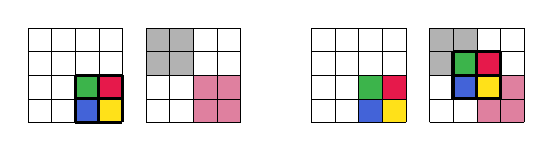
\begin{tikzpicture}[scale=0.3]
        \foreach \line [count=\y] in \gridpix {
            \foreach \pix [count=\x] in \line {
                \fill[color=pixel \pix] (-\x,-\y) rectangle +(1,1);
            }
        }
        \draw[very thick,step=1] (-2.0,-2.0) grid (0.0, 0.0);
        
        \draw[very thin,step=1] (-4.0,-2.0) grid (0.0, 2.0);
        
        \foreach \line [count=\y] in \gridpix {
            \foreach \pix [count=\x] in \line {
                \fill[color=black!30] (3-\x,2-\y) rectangle +(1,1);
            }
        }
        \foreach \line [count=\y] in \gridpix {
            \foreach \pix [count=\x] in \line {
                \fill[color=purple!50] (5-\x,-\y) rectangle +(1,1);
            }
        }

        \foreach \line [count=\y] in \gridpix {
            \foreach \pix [count=\x] in \line {
                \fill[color=pixel \pix] (12-\x,-\y) rectangle +(1,1);
            }
        }
        \draw[very thin,step=1] (1.0,-2.0) grid (5.0, 2.0);
        
        \draw[very thin,step=1] (8.0,-2.0) grid (12.0, 2.0);

        \foreach \line [count=\y] in \gridpix {
            \foreach \pix [count=\x] in \line {
                \fill[color=black!30] (15-\x,2-\y) rectangle +(1,1);
            }
        }
        \foreach \line [count=\y] in \gridpix {
            \foreach \pix [count=\x] in \line {
                \fill[color=purple!50] (17-\x,-\y) rectangle +(1,1);
            }
        }
        \foreach \line [count=\y] in \gridpix {
            \foreach \pix [count=\x] in \line {
                \fill[color=pixel \pix] (16-\x,1-\y) rectangle +(1,1);
            }
        }

        \draw[very thick,step=1] (14.0,-1.0) grid (16.0, 1.0);
        \draw[very thin,step=1] (13.0,-2.0) grid (17.0, 2.0);
    \end{tikzpicture}
    \caption{{\em Performing a blit from a \(2\times 2\) subgrid to another \(2\times 2\) subgrid, each in distinct grids. }}
    \label{fig:enter-label}
\end{figure}

Note the following:
\begin{itemize}
    \item only part of the grid gets moved,
    \item the blitted subgrid doesn't necessarily maintain its positioning, and
    \item the relative positioning of the cells in the blitted subgrid remains the same.
\end{itemize}

Let $n$ be a power of two. In this problem, we are given an $n \times n$ pixel map and our goal is to rotate the map $90^{\circ}$ clockwise.

\begin{figure}[H]
    \centering
    \scalebox{0.9}{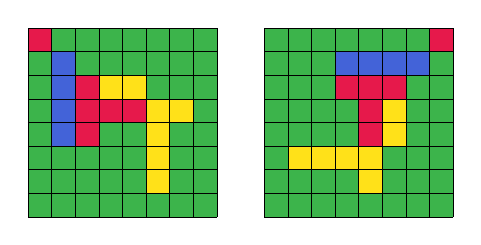
\begin{tikzpicture}[scale = 0.3]
        \foreach \line [count=\y] in \pixels {
            \foreach \pix [count=\x] in \line {
              \fill[color=pixel \pix] (\x,-\y) rectangle +(1,1);
            }
          }
          \draw[ultra thin,step=1] (1,-8) grid ++(8,8);

          \foreach \line [count=\y] in \pixel {
            \foreach \pix [count=\x] in \line {
              \fill[color=pixel \pix, xshift = 10cm] (\x,-\y) rectangle +(1,1);
            }
          }
          \draw[ultra thin,step=1] (11,-8) grid ++(8,8);
    \end{tikzpicture}}
    \caption{{\em Rotating the pixel map $90^{\circ}$ clockwise.}}
    \label{fig:enter-label}
\end{figure}

Design and analyse an algorithm which runs in $O(n^2)$ time and outputs a sequence of $O(n^2)$ blit operations to rotate a pixel map $90^{\circ}$ clockwise. You do not need to explicitly give the sequence; instead, show how the sequence is constructed and collected. You may assume that $\Theta(n^2)$ temporary space is available for you to transfer and cache subgrids.

\end{question}
\begin{rubric}
\begin{itemize}
    \item Your response should describe the steps followed to execute the algorithm in simple English. Do not write a program, and do not transcribe a program back to written English.
    
    You \textbf{must} justify the correctness of your algorithm.
    
    You \textbf{must} justify that your algorithm runs in time complexity that you claim.

    \item Course materials such as lectures and tutorials don't require attribution, but making explicit reference to similar ideas is still helpful to show your understanding.
\end{itemize}
Expected response length: less than one page.
\end{rubric}

\begin{solution}
\end{solution}

\begin{attribution}
\end{attribution}

\end{document}